\documentclass[11pt]{article}

\usepackage[a4paper,margin=2.7cm]{geometry}
\usepackage[T1]{fontenc}
\usepackage[utf8]{inputenc}
\usepackage{lmodern}
\usepackage{microtype}
\usepackage{amsmath,amssymb,amsthm,mathtools,bm}
\usepackage{booktabs,array,longtable}
\usepackage{graphicx}
\usepackage{caption}
\usepackage{subcaption}
\usepackage{enumitem}
\usepackage[backend=biber,style=authoryear,natbib=true,maxcitenames=2,maxbibnames=99]{biblatex}
\addbibresource{references.bib}
\usepackage{xcolor}
\usepackage[hidelinks]{hyperref}
\usepackage[nameinlink,noabbrev]{cleveref}

\setlength{\parindent}{1.2em}
\setlength{\parskip}{0.25em}
\setlist{nosep,leftmargin=2em}

\newtheorem{theorem}{Theorem}[section]
\newtheorem{proposition}[theorem]{Proposition}
\newtheorem{corollary}[theorem]{Corollary}
\newtheorem{lemma}[theorem]{Lemma}
\newtheorem{assumption}[theorem]{Assumption}
\theoremstyle{definition}
\newtheorem{definition}[theorem]{Definition}
\newtheorem{remark}[theorem]{Remark}

\newcommand{\R}{\mathbb{R}}
\newcommand{\E}{\mathbb{E}}
\newcommand{\Pp}{\mathbb{P}}
\newcommand{\Var}{\operatorname{Var}}
\newcommand{\Cov}{\operatorname{Cov}}
\newcommand{\tr}{\operatorname{tr}}
\newcommand{\diag}{\operatorname{diag}}
\newcommand{\op}{o_{\Pp}}
\newcommand{\Op}{O_{\Pp}}
\newcommand{\Normal}{\mathcal{N}}
\newcommand{\ThetaSet}{\boldsymbol{\Theta}}
\newcommand{\thetao}{\theta_0}
\newcommand{\phik}{\varphi_K}
\newcommand{\BS}{Brandt and Santa-Clara}

\title{\textbf{Euler-Based Simulated Likelihood for Multidimensional Diffusions:}\\
Dimensional Variance, Joint Asymptotics, and an Application Revisited}
\author{Diogo\\[0.3em]\small Draft for mathematical review}
\date{26 July 2026}

\begin{document}
\maketitle

\begin{abstract}
A widely used simulation method for likelihood inference in discretely observed diffusions approximates each transition density by simulating an Euler scheme to one time step before the observed endpoint and averaging the final Gaussian transition density. We show that this endpoint estimator is a shrinking-bandwidth kernel estimator whose Monte Carlo variance increases with the Euler discretisation level at a dimension-dependent rate. For a $K$-dimensional uniformly elliptic diffusion, its one-simulation second moment is generically of order $M^{K/2}$, where $M$ is the number of Euler substeps. Hence its variance is of order $M^{K/2}/S$, not uniformly of order $1/S$, where $S$ is the number of simulations. In the exact Brownian benchmark we derive all moments, establish the corrected central-limit normalisation, and construct a direct joint-limit counterexample. In four dimensions, the condition $\sqrt{S}/M\to0$ stated by \citet{BrandtSantaClara2002} is equivalent to $S/M^2\to0$, whereas mean-square consistency of the simulated density requires $S/M^2\to\infty$. Along the admissible sequence $M=S\to\infty$, the estimator converges in probability to zero although the true density is strictly positive. We derive the resulting bias--variance trade-off, the optimal pointwise rate, and the scale of the nonlinear log-likelihood error. We then examine the proof structure and the mathematical status of the exchange-rate application, including square-root boundaries, an implicitly defined volatility process, positive-semidefiniteness of the Brownian correlation matrix, minimum-incompleteness identification, and binding inequality constraints. The paper distinguishes a false joint asymptotic statement from proof gaps and from assumptions that do not cover the empirical model. It does not assert that the published numerical estimates are necessarily incorrect; it establishes that their stated asymptotic justification is incomplete and, in the four-dimensional case, contradicted by an exact counterexample.
\end{abstract}

\noindent\textbf{Keywords:} simulated maximum likelihood; diffusion processes; Euler scheme; transition density; Monte Carlo variance; curse of dimensionality; diffusion bridges; nonregular inference.

\noindent\textbf{JEL classifications:} C13; C15; C32; G12; G15.

\section{Introduction}

Continuous-time diffusion models are often observed only at discrete dates. Their exact transition densities are rarely available, which makes exact maximum likelihood difficult even when simulation of approximate sample paths is straightforward. One influential response is the simulation method introduced by \citet{Pedersen1995a,Pedersen1995b} and developed and applied by \citet{BrandtSantaClara2002}. The method divides each observation interval into $M$ Euler substeps, simulates the process through the first $M-1$ steps, evaluates the Gaussian density of the final Euler step at the observed endpoint, and averages this density over $S$ simulated paths.

For fixed $M$, the construction is elementary: the sample average converges to the transition density of the $M$-step Euler chain as $S\to\infty$. For fixed $S$ it is also clear that making the final time step smaller turns the Gaussian endpoint density into an increasingly narrow and increasingly high function. The mathematical question is therefore not whether the two separate approximations are individually meaningful. It is whether they remain compatible when $M$ and $S$ increase jointly.

The central observation of this paper is that the final Gaussian density is a kernel with bandwidth $h^{1/2}$, where $h=1/M$. In $K$ dimensions its effective volume is of order $h^{K/2}$ and its height is of order $h^{-K/2}$. Only simulations that fall in a shrinking neighbourhood of the endpoint contribute materially. The effective number of such simulations is therefore of order
\[
S h^{K/2}=\frac{S}{M^{K/2}}.
\]
This quantity, rather than $S$ alone, controls the Monte Carlo approximation.

The paper makes six main contributions.

First, we derive exact finite-$M$ moments for the estimator under $K$-dimensional Brownian motion. The Euler approximation is exact in this benchmark, so any failure is caused by the endpoint Monte Carlo construction and not by discretisation bias, boundary behaviour, nonlinear coefficients, or parameter identification.

Second, we construct a direct counterexample to the joint convergence result stated in Lemma 2 and Theorem 1 of \citet{BrandtSantaClara2002}. For every $K>2$, choosing $M=S=n$ makes the simulated density at the Brownian origin converge in probability to zero. This sequence satisfies the paper's condition $\sqrt{S}/M\to0$. In the four-dimensional application, their condition requires $S/M^2\to0$, while the variance calculation requires $S/M^2\to\infty$ for mean-square consistency.

Third, we establish the generic local moment law for a smooth uniformly elliptic diffusion. If $G_h$ denotes one endpoint-density summand, then for $r>1$,
\[
h^{(r-1)K/2}\E[G_h^r]
\longrightarrow
(2\pi)^{-(r-1)K/2}r^{-K/2}
 p(y\mid x)|V(y)|^{-(r-1)/2}.
\]
In particular, $\Var(G_h)$ is of order $h^{-K/2}$. This gives the corrected triangular-array central-limit normalisation
\[
\sqrt{S h^{K/2}}\,\bigl(\widehat q_{M,S}-q_M\bigr),
\]
not $\sqrt{S}(\widehat q_{M,S}-q_M)$.

Fourth, we combine the $O(M^{-1})$ Euler density bias used by \citet{BrandtSantaClara2002} with the corrected simulation variance. The resulting pointwise mean squared error is
\[
O(M^{-2})+O\!\left(\frac{M^{K/2}}{S}\right),
\]
which is minimised at $M\asymp S^{2/(K+4)}$ and yields the rate $S^{-4/(K+4)}$. The estimator therefore exhibits an explicit curse of dimensionality.

Fifth, we trace the density-level result into the log likelihood. The nonlinearity of the logarithm operates on the effective Monte Carlo size $S/M^{K/2}$. Whenever a standard second-order delta expansion is valid, the leading log-density bias is of order $M^{K/2}/S$, rather than uniformly of order $1/S$. This distinction matters because simulated likelihood sums a log transformation over all observations.

Sixth, we examine the mathematical status of the exchange-rate application. The empirical model contains square-root diffusions that violate the smoothness and nondegeneracy assumptions of the generic theorem. The market-incompleteness state reaches a degenerate boundary and ordinary Euler discretisation is not positivity preserving. The time-varying risk-price specification defines exchange-rate volatility through an implicit quadratic identity, and the reported U.S.--U.K. estimates fail a natural sufficient condition for a unique positive volatility branch. The full Brownian correlation matrix requires a joint positive-semidefinite constraint, not merely pairwise correlations in $[-1,1]$. Finally, the minimum-incompleteness identification rule and the binding nonnegativity constraint lead to a hybrid and potentially nonregular estimator not covered by the unconstrained SML theorem.

The aim is not to relitigate the substantive economics of a paper published more than two decades ago. Nor do we infer from a false theorem that every numerical estimate obtained with finite $M$ and $S$ must be poor. The aim is narrower and mathematical: to identify the correct dimensional scale of the endpoint estimator, separate sequential from joint convergence, and determine what the published asymptotic arguments do and do not establish.

The remainder is organised as follows. \Cref{sec:estimator} defines the estimator. \Cref{sec:brownian} gives exact Brownian results and the counterexample. \Cref{sec:general} derives the general diffusion moment law and corrected CLT. \Cref{sec:mse} studies the bias--variance trade-off. \Cref{sec:loglik} discusses log likelihood and parameter estimation. \Cref{sec:proof_review} analyses the published proof. \Cref{sec:application} studies the exchange-rate diffusion. \Cref{sec:numerics} presents reproducible numerical evidence, and \Cref{sec:remedies} discusses variance-reduction alternatives.

\section{The endpoint simulated-likelihood estimator}\label{sec:estimator}

Let $Y_t\in\R^K$ satisfy the stochastic differential equation
\begin{equation}\label{eq:sde}
 dY_t=\mu(Y_t,t;\theta)\,dt+\Sigma(Y_t,t;\theta)\,dW_t,
 \qquad V=\Sigma\Sigma^{\mathsf T},
\end{equation}
where $W_t$ is a Brownian motion of suitable dimension and $\theta\in\ThetaSet\subset\R^L$. We suppress $t$ and $\theta$ where no ambiguity arises. Consider one observation interval of length one, from $Y_0=x$ to $Y_1=y$. The normalisation to unit length is only notational.

For $M\ge2$, set $h=1/M$ and define the Euler chain
\begin{equation}\label{eq:euler}
Y^M_{m+1}=Y^M_m+\mu(Y^M_m,mh)h
 +\Sigma(Y^M_m,mh)\sqrt{h}\,\varepsilon_{m+1},
\qquad m=0,\ldots,M-1,
\end{equation}
with $Y^M_0=x$ and independent $\varepsilon_m\sim\Normal(0,I)$. Conditional on $Y^M_m=z$, the one-step density is
\begin{equation}\label{eq:one_step_kernel}
g_h(y\mid z)
=
\phik\!\left(y;
 z+\mu(z,1-h)h,
 hV(z,1-h)
\right).
\end{equation}
Let $Z_h=Y^M_{M-1}$ denote the preterminal Euler state and let $r_h(z\mid x)$ be its density. The $M$-step Euler transition density is
\begin{equation}\label{eq:euler_density_expectation}
q_M(y\mid x)=\E[g_h(y\mid Z_h)]
=\int_{\R^K}g_h(y\mid z)r_h(z\mid x)\,dz.
\end{equation}

The endpoint simulation estimator is
\begin{equation}\label{eq:pedersen_estimator}
\widehat q_{M,S}(y\mid x)
=
\frac{1}{S}\sum_{s=1}^S g_h(y\mid Z_{h,s}),
\end{equation}
where $Z_{h,1},\ldots,Z_{h,S}$ are independent draws from the preterminal Euler law. This is equation (8) of \citet{BrandtSantaClara2002}, with notation adapted to the present analysis.

For each fixed $M$, the strong law yields
\[
\widehat q_{M,S}(y\mid x)\longrightarrow q_M(y\mid x)
\quad\text{almost surely as }S\to\infty,
\]
provided the summand is integrable. Under regularity conditions such as those of \citet{BallyTalay1995,BallyTalay1996},
\[
q_M(y\mid x)-p(y\mid x)=O(M^{-1}),
\]
where $p$ is the diffusion transition density. These two facts establish a sequential limit: first $S\to\infty$ for fixed $M$, then $M\to\infty$. They do not establish convergence along arbitrary joint sequences $M,S\to\infty$.

The geometry of \eqref{eq:one_step_kernel} explains why. Its covariance is $hV(z)$. Under nondegeneracy, it is concentrated in a ball of radius $O(\sqrt h)$ around the endpoint and has maximum height $O(h^{-K/2})$. The integral in \eqref{eq:euler_density_expectation} remains finite because the effective volume is $O(h^{K/2})$. A Monte Carlo average resolves that integral only if enough preterminal draws enter this shrinking region.

\begin{definition}[Effective endpoint simulation size]\label{def:effective_size}
For a $K$-dimensional endpoint estimator with Euler step $h=1/M$, define
\begin{equation}\label{eq:effective_size}
R_{M,S}=S h^{K/2}=\frac{S}{M^{K/2}}.
\end{equation}
This is the expected-order number of simulations falling in an $O(\sqrt h)$ neighbourhood of an endpoint with a regular positive preterminal density.
\end{definition}

The next sections make this interpretation exact.

\section{Exact Brownian analysis}\label{sec:brownian}

Consider standard Brownian motion in $\R^K$,
\begin{equation}\label{eq:brownian}
dY_t=dW_t,
\end{equation}
observed over a unit interval. Euler discretisation is exact. Set $Y_0=x$ and evaluate the transition density at $Y_1=y$. With $h=1/M$,
\[
Z_h\sim\Normal(x,(1-h)I_K)
\]
and a single endpoint summand is
\begin{equation}\label{eq:brownian_summand}
G_h
=(2\pi h)^{-K/2}
\exp\!\left[-\frac{\|y-Z_h\|^2}{2h}\right].
\end{equation}

\subsection{Exact moments}

\begin{proposition}[Exact Brownian moments]\label{prop:brownian_moments}
Let $r>0$. For the summand \eqref{eq:brownian_summand},
\begin{align}
\E[G_h^r]
&=(2\pi h)^{-rK/2}
\left(1+\frac{r(1-h)}{h}\right)^{-K/2}
\exp\!\left[
-\frac{r\|y-x\|^2}{2\{h+r(1-h)\}}
\right] \label{eq:brownian_r_moment}\\
&=(2\pi)^{-rK/2}
 h^{-(r-1)K/2}
\{r-(r-1)h\}^{-K/2}
\exp\!\left[
-\frac{r\|y-x\|^2}{2\{r-(r-1)h\}}
\right]. \nonumber
\end{align}
In particular,
\begin{equation}\label{eq:brownian_mean}
\E[G_h]=(2\pi)^{-K/2}\exp\!\left[-\frac{\|y-x\|^2}{2}\right]
=p(y\mid x),
\end{equation}
and
\begin{equation}\label{eq:brownian_second}
\E[G_h^2]
=(2\pi)^{-K}h^{-K/2}(2-h)^{-K/2}
\exp\!\left[-\frac{\|y-x\|^2}{2-h}\right].
\end{equation}
\end{proposition}

\begin{proof}
For $Z\sim\Normal(x,(1-h)I_K)$ and $c>0$, the Gaussian identity
\[
\E\!\left[e^{-c\|Z-y\|^2}\right]
=\{1+2c(1-h)\}^{-K/2}
\exp\!\left[-\frac{c\|x-y\|^2}{1+2c(1-h)}\right]
\]
follows by completing the square. Apply it with $c=r/(2h)$ and multiply by the prefactor $(2\pi h)^{-rK/2}$. The cases $r=1$ and $r=2$ follow directly.
\end{proof}

\begin{corollary}[Exact variance]\label{cor:brownian_variance}
For $S$ independent simulations,
\begin{equation}\label{eq:brownian_estimator_variance}
\Var(\widehat q_{M,S})
=
\frac{1}{S}\left[
(2\pi)^{-K}h^{-K/2}(2-h)^{-K/2}
 e^{-\|y-x\|^2/(2-h)}
-p(y\mid x)^2
\right].
\end{equation}
Hence
\begin{equation}\label{eq:brownian_variance_asymptotic}
\Var(\widehat q_{M,S})
\sim
\frac{\tau_K^2(x,y)}{S h^{K/2}},
\qquad
\tau_K^2(x,y)
=(2\pi)^{-K}2^{-K/2}e^{-\|y-x\|^2/2}.
\end{equation}
\end{corollary}

The variance is not uniformly $O(1/S)$. It is $O(M^{K/2}/S)$. The estimator is unbiased in this example for every $M$, but its distribution becomes increasingly dominated by rare, very large contributions when $R_{M,S}$ is small.

\subsection{A direct joint-limit counterexample}

A variance calculation alone does not prove failure of convergence in probability because a non-uniformly integrable sequence can converge in probability while retaining large or divergent moments. The next theorem gives a direct failure result.

\begin{theorem}[Collapse along $M=S$]\label{thm:collapse}
Let $K>2$, $x=y=0$, and choose $M_n=S_n=n$. Then the Brownian endpoint estimator satisfies
\begin{equation}\label{eq:collapse}
\widehat q_{n,n}(0\mid0)\longrightarrow0
\qquad\text{in probability},
\end{equation}
although
\[
p(0\mid0)=(2\pi)^{-K/2}>0.
\]
For $K=4$, the sequence satisfies the rate condition
\[
\frac{\sqrt{S_n}}{M_n}=n^{-1/2}\longrightarrow0
\]
used in Theorems 1 and 2 of \citet{BrandtSantaClara2002}.
\end{theorem}

\begin{proof}
Write $h_n=1/n$ and let $Z_{n,1},\ldots,Z_{n,n}$ be the preterminal draws, each distributed as $\Normal(0,(1-1/n)I_K)$. Fix a constant $c>K$ and define
\[
r_n=\sqrt{\frac{c\log n}{n}}.
\]
Let $A_n$ be the event that at least one draw lies in the ball $B(0,r_n)$. The Gaussian densities of the $Z_{n,s}$ are uniformly bounded for $n\ge2$, so for a constant $C_K$,
\[
\Pp(A_n)
\le n\Pp(\|Z_{n,1}\|\le r_n)
\le C_K n r_n^K
=C_Kc^{K/2}n^{1-K/2}(\log n)^{K/2}
\longrightarrow0
\]
because $K>2$.

On $A_n^c$, every summand is bounded by
\[
\left(\frac{n}{2\pi}\right)^{K/2}
\exp\!\left(-\frac{nr_n^2}{2}\right)
=(2\pi)^{-K/2}n^{(K-c)/2},
\]
which tends to zero because $c>K$. The sample average obeys the same bound. Therefore, for every $\varepsilon>0$,
\[
\Pp(\widehat q_{n,n}>\varepsilon)
\le \Pp(A_n)+
\mathbf{1}\!\left\{(2\pi)^{-K/2}n^{(K-c)/2}>\varepsilon\right\}
\longrightarrow0.
\]
\end{proof}

\begin{remark}[How an unbiased estimator converges to zero]
For every $n$, $\E[\widehat q_{n,n}]=p(0\mid0)$. The convergence in probability to zero is sustained by increasingly rare simulations with increasingly large endpoint densities. The sequence is not uniformly integrable. This is precisely the rare-event geometry hidden by a fixed-$M$ application of the strong law.
\end{remark}

\begin{corollary}[Contradiction in four dimensions]\label{cor:contradiction}
For $K=4$, mean-square consistency requires
\[
\frac{S}{M^2}\longrightarrow\infty,
\]
whereas the published condition $\sqrt S/M\to0$ is equivalent to
\[
\frac{S}{M^2}\longrightarrow0.
\]
The two conditions are mutually exclusive. Moreover, \Cref{thm:collapse} shows that the published condition permits a sequence along which the density estimator converges to the wrong value.
\end{corollary}

\subsection{Correct triangular-array central limit theorem}

\begin{theorem}[Brownian endpoint CLT]\label{thm:brownian_clt}
Let $M\to\infty$ and $S\to\infty$ such that
\begin{equation}\label{eq:effective_diverge}
S h^{K/2}=\frac{S}{M^{K/2}}\longrightarrow\infty.
\end{equation}
Then
\begin{equation}\label{eq:brownian_clt}
\sqrt{S h^{K/2}}
\left\{\widehat q_{M,S}(y\mid x)-p(y\mid x)\right\}
\Longrightarrow
\Normal\!\left(0,\tau_K^2(x,y)\right),
\end{equation}
where $\tau_K^2(x,y)$ is defined in \eqref{eq:brownian_variance_asymptotic}.
\end{theorem}

\begin{proof}
Within each row, the $G_h$ are independent and identically distributed. By \Cref{prop:brownian_moments},
\[
\Var(G_h)\sim \tau_K^2 h^{-K/2},
\qquad
\E[|G_h|^3]=O(h^{-K}).
\]
The same order holds for the third absolute centred moment. The Lyapunov ratio is therefore
\[
\frac{S\E|G_h-\E G_h|^3}
{\{S\Var(G_h)\}^{3/2}}
=O\!\left(\frac{1}{\sqrt{S h^{K/2}}}\right)
\longrightarrow0.
\]
The triangular-array Lyapunov central limit theorem applies. The variance normalisation follows from \eqref{eq:brownian_variance_asymptotic}, and the Euler bias is zero for Brownian motion.
\end{proof}

The correct normalisation depends on dimension. A fixed-$M$ $\sqrt S$-CLT is valid, but it is not stable as $M\to\infty$.

\section{General multidimensional diffusions}\label{sec:general}

The Brownian calculation reflects a local property of Gaussian endpoint kernels. We now derive the generic moment law. The assumptions below are deliberately stronger than necessary so that the mechanism is transparent.

Let $G_h=g_h(y\mid Z_h)$ be one summand in \eqref{eq:pedersen_estimator}. Fix $x$ and $y$.

\begin{assumption}[Local regularity and domination]\label{ass:local}
As $h\downarrow0$:
\begin{enumerate}[label=(\roman*)]
\item $\mu(z)$ and $V(z)$ are continuous in a neighbourhood of $y$, and $V(y)$ is positive definite;
\item on that neighbourhood, the eigenvalues of $V(z)$ are bounded between constants $0<\underline v<\overline v<\infty$ and $\mu$ is bounded;
\item the preterminal Euler density $r_h(z\mid x)$ converges locally uniformly at $y$ to a continuous density $p(z\mid x)$, with $p(y\mid x)>0$;
\item the family $r_h(\cdot\mid x)$ is uniformly bounded and the contribution to the moment integral from outside any fixed neighbourhood of $y$ is dominated by an integrable Gaussian envelope after multiplication by the appropriate power of $h$.
\end{enumerate}
\end{assumption}

Uniform ellipticity, bounded smooth coefficients, and standard Gaussian density bounds imply versions of these conditions. They are compatible with the regular setting used to justify Euler density expansions in \citet{BallyTalay1995,BallyTalay1996}. They are not compatible with the square-root boundaries in the later financial application; that distinction is discussed in \Cref{sec:application}.

\begin{theorem}[Local moment law]\label{thm:local_moments}
Under \Cref{ass:local}, for every fixed $r>1$,
\begin{equation}\label{eq:general_r_moment}
 h^{(r-1)K/2}\E[G_h^r]
\longrightarrow
c_{r,K}\,p(y\mid x)\,|V(y)|^{-(r-1)/2},
\end{equation}
where
\begin{equation}\label{eq:crk}
c_{r,K}=(2\pi)^{-(r-1)K/2}r^{-K/2}.
\end{equation}
In particular,
\begin{equation}\label{eq:general_second}
 h^{K/2}\E[G_h^2]
\longrightarrow
(4\pi)^{-K/2}p(y\mid x)|V(y)|^{-1/2}.
\end{equation}
\end{theorem}

\begin{proof}
Write $z=y+\sqrt h\,u$. On a fixed neighbourhood of $y$,
\begin{align*}
G_h^r
&=(2\pi h)^{-rK/2}|V(z)|^{-r/2}\\
&\quad\times
\exp\!\left[-\frac{r}{2h}
\{y-z-h\mu(z)\}^{\mathsf T}V(z)^{-1}
\{y-z-h\mu(z)\}\right].
\end{align*}
Since $dz=h^{K/2}du$, multiplication by $h^{(r-1)K/2}$ cancels the powers of $h$. Pointwise in $u$,
\[
V(y+\sqrt h\,u)\to V(y),
\qquad
r_h(y+\sqrt h\,u\mid x)\to p(y\mid x),
\]
and the exponent converges to
\[
-\frac r2u^{\mathsf T}V(y)^{-1}u.
\]
The local eigenvalue bounds give an integrable Gaussian envelope. Dominated convergence and the tail condition yield
\begin{align*}
&\lim_{h\downarrow0}h^{(r-1)K/2}\E[G_h^r]\\
&\quad=(2\pi)^{-rK/2}|V(y)|^{-r/2}p(y\mid x)
\int_{\R^K}\exp\!\left[-\frac r2u^{\mathsf T}V(y)^{-1}u\right]du\\
&\quad=(2\pi)^{-rK/2}|V(y)|^{-r/2}p(y\mid x)
(2\pi/r)^{K/2}|V(y)|^{1/2},
\end{align*}
which is \eqref{eq:general_r_moment}.
\end{proof}

\begin{corollary}[Generic variance scale]\label{cor:generic_variance}
Let $q_M(y\mid x)=\E[G_h]$ and suppose $q_M(y\mid x)\to p(y\mid x)$. Then
\begin{equation}\label{eq:generic_variance}
\Var(\widehat q_{M,S})
\sim
\frac{\tau^2(x,y)}{S h^{K/2}},
\qquad
\tau^2(x,y)=(4\pi)^{-K/2}p(y\mid x)|V(y)|^{-1/2}.
\end{equation}
\end{corollary}

\begin{theorem}[Generic endpoint CLT]\label{thm:generic_clt}
Under \Cref{ass:local}, if $S h^{K/2}\to\infty$, then
\begin{equation}\label{eq:generic_clt}
\sqrt{S h^{K/2}}
\left\{\widehat q_{M,S}(y\mid x)-q_M(y\mid x)\right\}
\Longrightarrow
\Normal(0,\tau^2(x,y)).
\end{equation}
\end{theorem}

\begin{proof}
The $r=2$ and $r=3$ cases of \Cref{thm:local_moments} imply
\[
\Var(G_h)\sim\tau^2h^{-K/2},
\qquad
\E|G_h-\E G_h|^3=O(h^{-K}).
\]
The Lyapunov ratio is again $O\{(S h^{K/2})^{-1/2}\}$.
\end{proof}

\begin{corollary}[CLT centred at the diffusion density]\label{cor:diffusion_clt}
Suppose in addition that
\begin{equation}\label{eq:euler_bias_expansion}
q_M(y\mid x)-p(y\mid x)=b(x,y)h+o(h).
\end{equation}
If
\begin{equation}\label{eq:bias_negligible}
S h^{K/2}\to\infty,
\qquad
\sqrt{S h^{K/2}}\,h\to0,
\end{equation}
then
\begin{equation}\label{eq:diffusion_clt}
\sqrt{S h^{K/2}}
\left\{\widehat q_{M,S}(y\mid x)-p(y\mid x)\right\}
\Longrightarrow
\Normal(0,\tau^2(x,y)).
\end{equation}
In terms of $M$ and $S$, the second condition is
\begin{equation}\label{eq:correct_bias_rate}
\frac{\sqrt S}{M^{1+K/4}}\longrightarrow0.
\end{equation}
For $K=4$, a feasible regime is
\begin{equation}\label{eq:k4_feasible}
M^2\ll S\ll M^4.
\end{equation}
\end{corollary}

\begin{remark}[The dimensional conflict]
The condition $\sqrt S/M\to0$ suppresses an $O(M^{-1})$ Euler bias under an incorrectly fixed Monte Carlo scale. Once the variance inflation $M^{K/2}$ is included, the bias must be compared with the standard deviation $M^{K/4}/\sqrt S$, producing \eqref{eq:correct_bias_rate}. In four dimensions, the lower consistency requirement and the upper bias requirement leave the nonempty interval \eqref{eq:k4_feasible}. The published condition places $S$ below the lower boundary of that interval.
\end{remark}

\section{Bias--variance trade-off and dimensional rate}\label{sec:mse}

Suppose the Euler density admits \eqref{eq:euler_bias_expansion}. Because \eqref{eq:pedersen_estimator} is unbiased for $q_M$,
\begin{align}
\E\!\left[(\widehat q_{M,S}-p)^2\right]
&=(q_M-p)^2+\Var(\widehat q_{M,S}) \nonumber\\
&=b(x,y)^2h^2
+\frac{\tau^2(x,y)}{S h^{K/2}}
+o\!\left(h^2+\frac{1}{S h^{K/2}}\right). \label{eq:mse_expansion}
\end{align}

\begin{proposition}[Pointwise optimal discretisation]\label{prop:optimal_m}
If $b(x,y)\ne0$, the leading terms in \eqref{eq:mse_expansion} are balanced by
\begin{equation}\label{eq:optimal_h}
h\asymp S^{-2/(K+4)},
\qquad
M\asymp S^{2/(K+4)}.
\end{equation}
The resulting optimal pointwise mean squared error is
\begin{equation}\label{eq:optimal_mse}
\operatorname{MSE}_{\mathrm{opt}}
\asymp S^{-4/(K+4)}.
\end{equation}
\end{proposition}

\begin{proof}
Differentiate the leading expression $B h^2+C/(S h^{K/2})$ with respect to $h$ or equate its two terms. This gives $h^{K/2+2}\asymp S^{-1}$ and hence \eqref{eq:optimal_h}. Substitution yields \eqref{eq:optimal_mse}.
\end{proof}

The rate is the familiar structure of a kernel-density problem: reducing the bandwidth controls approximation bias but decreases the effective number of simulations. The dimension enters through the volume of the final Gaussian kernel. Some illustrative exponents are
\begin{center}
\begin{tabular}{ccc}
\toprule
Dimension $K$ & $M_{\mathrm{opt}}$ & Optimal MSE \\
\midrule
$1$ & $S^{2/5}$ & $S^{-4/5}$ \\
$2$ & $S^{1/3}$ & $S^{-2/3}$ \\
$4$ & $S^{1/4}$ & $S^{-1/2}$ \\
$8$ & $S^{1/6}$ & $S^{-1/3}$ \\
\bottomrule
\end{tabular}
\end{center}

This does not mean that $M$ should always be chosen by pointwise MSE. Likelihood estimation requires accuracy over many endpoints and parameter values, and higher-order or bridge-based methods can change both constants and rates. It does mean that increasing $M$ while holding $S$ fixed, or while letting $S$ grow too slowly relative to dimension, can make the simulation approximation worse rather than better.

\begin{table}[t]
\centering
\caption{Principal endpoint-density rate conditions.}
\label{tab:rates}
\begin{tabular}{lll}
\toprule
Property & General dimension $K$ & Four dimensions \\
\midrule
Monte Carlo mean-square consistency
& $S/M^{K/2}\to\infty$ & $S/M^2\to\infty$ \\
Density CLT centred at $q_M$
& $S/M^{K/2}\to\infty$ & $S/M^2\to\infty$ \\
Euler bias negligible in corrected CLT
& $\sqrt S/M^{1+K/4}\to0$ & $S/M^4\to0$ \\
Condition in \citet{BrandtSantaClara2002}
& $\sqrt S/M\to0$ & $S/M^2\to0$ \\
\bottomrule
\end{tabular}
\end{table}

\section{From density error to log-likelihood error}\label{sec:loglik}

For observations $Y_0,\ldots,Y_N$, the simulated log likelihood is a sum of terms
\[
\log\widehat q_{M,S}(Y_{n+1}\mid Y_n;\theta).
\]
Even when $\widehat q_{M,S}$ is unbiased for $q_M$, its logarithm is not unbiased. The effective endpoint size $R_{M,S}=S h^{K/2}$ controls this nonlinearity.

\begin{proposition}[Log-density delta expansion]\label{prop:log_delta}
Fix an endpoint with $q_M\to p>0$ and suppose the conditions of \Cref{thm:generic_clt} hold. If $R_{M,S}=S h^{K/2}\to\infty$, then
\begin{equation}\label{eq:log_clt}
\sqrt{R_{M,S}}
\left\{\log\widehat q_{M,S}-\log q_M\right\}
\Longrightarrow
\Normal\!\left(0,\frac{\tau^2}{p^2}\right),
\end{equation}
and
\begin{equation}\label{eq:log_stochastic_expansion}
\log\widehat q_{M,S}-\log q_M
=
\frac{\widehat q_{M,S}-q_M}{q_M}
-\frac{(\widehat q_{M,S}-q_M)^2}{2q_M^2}
+\op(R_{M,S}^{-1}).
\end{equation}
Whenever the second-order expansion is uniformly integrable, it follows that
\begin{equation}\label{eq:log_bias}
\E[\log\widehat q_{M,S}]-\log q_M
=-\frac{\tau^2}{2p^2R_{M,S}}+o(R_{M,S}^{-1}).
\end{equation}
\end{proposition}

\begin{proof}
The first statement is the delta method applied to \Cref{thm:generic_clt}. Since $(\widehat q-q_M)/q_M=\Op(R^{-1/2})$ and $q_M$ is bounded away from zero, Taylor expansion of $\log(1+u)$ gives \eqref{eq:log_stochastic_expansion}. Taking expectations requires uniform integrability of the remainder and lower-tail control; under that additional condition, the first-order term has zero expectation and the second-order term gives \eqref{eq:log_bias}.
\end{proof}

The leading nonlinear scale is
\begin{equation}\label{eq:log_bias_order}
R_{M,S}^{-1}=\frac{M^{K/2}}{S},
\end{equation}
not uniformly $1/S$. The statement in \citet[p.~171]{BrandtSantaClara2002} that the logarithmic transformation induces a bias of order $1/S$ is valid with $M$ fixed. It is not a joint-$M,S$ order.

Suppose simulations are independent across observations and the local constants are uniformly bounded. For the average simulated criterion
\[
\widehat Q_{N,M,S}(\theta)
=\frac1N\sum_{n=0}^{N-1}
\log\widehat q_{n,M,S}(\theta),
\]
the stochastic average of the first-order simulation error has standard deviation of order
\[
(NR_{M,S})^{-1/2},
\]
while the average nonlinear bias remains of order $R_{M,S}^{-1}$. The simulation bias does not average out across observations.

A full estimator theorem requires uniform control in $\theta$ of densities, scores, and Hessians. The following standard perturbation statement separates those requirements from the endpoint calculations.

\begin{proposition}[Abstract equivalence to exact MLE]\label{prop:m_estimator}
Let $\widehat\theta_N$ maximise an exact average log likelihood $Q_N$, and let $\widehat\theta_{N,M,S}$ maximise a simulated criterion $\widehat Q_{N,M,S}$. Assume:
\begin{enumerate}[label=(\roman*)]
\item $\widehat\theta_N\to\thetao$ and $\sqrt N(\widehat\theta_N-\thetao)$ has the usual exact-MLE limit;
\item on a neighbourhood of $\thetao$,
\[
\sup_\theta
\|\nabla\widehat Q_{N,M,S}(\theta)-\nabla Q_N(\theta)\|
=o_{\Pp}(N^{-1/2});
\]
\item on the same neighbourhood,
\[
\sup_\theta
\|\nabla^2\widehat Q_{N,M,S}(\theta)-\nabla^2Q_N(\theta)\|
=o_{\Pp}(1);
\]
\item the exact criterion has a nonsingular limiting Hessian.
\end{enumerate}
Then
\[
\sqrt N(\widehat\theta_{N,M,S}-\widehat\theta_N)\to0
\quad\text{in probability}.
\]
\end{proposition}

\begin{proof}
Expand the simulated first-order condition around $\widehat\theta_N$ and use the uniform score and Hessian bounds together with nonsingularity of the limiting exact Hessian.
\end{proof}

Under uniform analogues of the pointwise density expansion, plausible minimum requirements for first-order equivalence include
\begin{equation}\label{eq:parameter_rate_heuristic}
S h^{K/2}\to\infty,
\qquad
\frac{\sqrt N}{S h^{K/2}}\to0,
\qquad
\sqrt N\,h\to0,
\end{equation}
corresponding respectively to vanishing score simulation noise, vanishing nonlinear simulation bias at the $N^{-1/2}$ scale, and negligible Euler bias. Derivatives of the simulated paths and Gaussian kernels can impose stronger conditions. Therefore \eqref{eq:parameter_rate_heuristic} is a design implication, not a claimed complete theorem for arbitrary diffusions.

The broader Monte Carlo likelihood literature treats joint data and simulation limits through empirical-process, importance-sampling, or exact-simulation arguments rather than by combining two pointwise limits; see, among others, \citet{Lee1995,SungGeyer2007,BeskosEtAl2009,MiasojedowEtAl2016}.

\section{What fails in the published asymptotic argument}\label{sec:proof_review}

This section distinguishes statements refuted by the Brownian example from steps that are merely unproved under the stated assumptions.

\subsection{Lemma 2: sequential convergence is used as joint convergence}

The proof of Lemma 2 in \citet{BrandtSantaClara2002} applies the strong law to the Monte Carlo average and then invokes convergence of the Euler density. For every fixed $M$,
\[
\widehat q_{M,S}\to q_M\quad\text{as }S\to\infty,
\]
and separately
\[
q_M\to p\quad\text{as }M\to\infty.
\]
This gives the iterated limit
\[
\lim_{M\to\infty}\lim_{S\to\infty}\widehat q_{M,S}=p.
\]
It does not give convergence along every sequence $(M_n,S_n)\to(\infty,\infty)$. The summand changes with $M$ and its variance diverges as $M^{K/2}$. \Cref{thm:collapse} directly refutes the stated joint conclusion.

\subsection{Lemma 3: the fixed-$M$ CLT is not uniform in $M$}

The paper uses a $\sqrt S$ central limit theorem and requires $\sqrt S/M\to0$ to suppress the Euler bias. The variance of the triangular-array summand is not asymptotically constant. It is of order $M^{K/2}$. The correct standardisation is $\sqrt{S/M^{K/2}}$. The Euler bias must then be compared with that scale, producing \eqref{eq:correct_bias_rate}.

\subsection{Lemma 4: an $O_{\Pp}$ term is treated as $o_{\Pp}$}

Let $x_n=\widehat q_n-p_n$. A nondegenerate central limit theorem implies $x_n=O_{\Pp}(S^{-1/2})$ for fixed $M$, not $o_{\Pp}(S^{-1/2})$. The Taylor expansion
\[
\log\left(1+\frac{x_n}{p_n}\right)
=\frac{x_n}{p_n}+O_{\Pp}(x_n^2)
\]
retains a first-order stochastic term. In the joint limit, the correct order is $O_{\Pp}\{(S h^{K/2})^{-1/2}\}$. Moreover, summing pointwise errors over $N$ observations requires lower bounds or tail control for $p_n$, dependence control, and a triangular-array argument. These are not supplied.

\subsection{Lemma 5: convergence of objective values does not control maximisers}

An argmax result requires uniform convergence of the criterion and separation or local curvature around the maximiser. A bounded Hessian gives an upper quadratic bound. To infer that two maximisers are close from a small objective difference, one needs a lower quadratic bound or a negative Hessian whose smallest eigenvalue is bounded away from zero after normalisation. Pointwise convergence and identification alone are insufficient.

\subsection{Lemmas 6 and 7: exact-MLE asymptotics require additional structure}

Consistency of the exact diffusion MLE ordinarily requires a uniform law of large numbers, global or local identification, and stability assumptions such as stationarity and ergodicity when $N\to\infty$. A score expansion around $\thetao$ is not by itself a proof of consistency because the intermediate Hessian is evaluated between the estimator and $\thetao$.

Similarly, a martingale CLT requires convergence of the realised conditional quadratic variation and a conditional Lindeberg condition. Defining Fisher information as an expectation does not make the realised conditional variance condition automatic. Boundedness of $\partial p/\partial\theta$ is also not a bound on the score $(\partial p/\partial\theta)/p$ when $p$ can be small.

These points do not imply that no correct exact-MLE theorem can be written. They imply that the short proof in Appendix A does not establish the stated result, even apart from the false transition-density joint limit.

\section{Mathematical status of the exchange-rate application}\label{sec:application}

The empirical application estimates a four-dimensional system consisting of two interest rates, the log exchange rate, and exchange-rate volatility. It also reconstructs a market-incompleteness state. Several mathematical features are not covered by the generic SML theorem.

\subsection{Square-root coefficients violate the generic assumptions}

The interest rates are modelled as correlated Cox--Ingersoll--Ross processes,
\begin{equation}\label{eq:cir_rates}
dr_t=\lambda(\vartheta-r_t)dt+\sigma\sqrt{r_t}\,dW_t,
\qquad
d r_t^*=\lambda^*(\vartheta^*-r_t^*)dt+\sigma^*\sqrt{r_t^*}\,dW_t^*.
\end{equation}
The generic theory assumes infinitely differentiable coefficients with bounded derivatives and a positive-definite covariance matrix. The function $r\mapsto\sqrt r$ is not differentiable at zero, has unbounded derivatives near zero, is not defined on the negative half-line as a real coefficient, and makes the covariance degenerate at the boundary.

The exact CIR process can preserve nonnegativity under its boundary conditions, but the ordinary Euler update
\[
r_{m+1}=r_m+\lambda(\vartheta-r_m)h
+\sigma\sqrt{r_mh}\,\varepsilon_{m+1}
\]
has a Gaussian conditional distribution and therefore a positive probability of becoming negative whenever its conditional variance is nonzero. A truncation, reflection, absorption, or exact-transition rule would define a different approximation and would require its own convergence analysis. The published paper does not specify such a rule.

The market-incompleteness state is even more direct. Let $X_t=\epsilon_t^2$. The model is
\begin{equation}\label{eq:epsilon_cir}
dX_t=(\beta^2-2\alpha X_t)dt+2\beta\sqrt{X_t}\,dY_t.
\end{equation}
This is a CIR process with $\kappa=2\alpha$, long-run mean $\beta^2/(2\alpha)$, and diffusion coefficient $2\beta$. Its Feller quantities satisfy
\[
2\kappa\vartheta=2\beta^2<4\beta^2=(2\beta)^2
\]
for every $\beta\ne0$. Hence zero is attainable, and the instantaneous covariance degenerates there. The generic positive-definiteness assumption therefore fails structurally, not only for an exceptional parameter value.

For an Euler step of size $h$, the probability of a negative next state from $X_t=x>0$ is
\begin{equation}\label{eq:negative_prob}
\Phi\!\left(
-\frac{x+(\beta^2-2\alpha x)h}{2\beta\sqrt{xh}}
\right).
\end{equation}
\Cref{fig:negative_euler} plots this probability using the estimates reported in Table 3 of \citet{BrandtSantaClara2002}. It can be material near the attainable boundary.

\subsection{The time-varying volatility specification is implicit}

The time-varying pure-currency risk prices have the form
\begin{equation}\label{eq:risk_price_v}
\psi_t=a_t+bv_t,
\qquad
\psi_t^*=a_t^*+b^*v_t,
\end{equation}
where $a_t$ and $a_t^*$ depend on the interest-rate differential and log exchange rate. The variance identity is
\begin{equation}\label{eq:vol_identity}
v_t^2
=D_t+\psi_t^2+(\psi_t^*)^2-2\rho\psi_t\psi_t^*,
\end{equation}
where $D_t$ collects the interest-rate risk term and $\epsilon_t^2$.

Substituting \eqref{eq:risk_price_v} into \eqref{eq:vol_identity} gives
\begin{equation}\label{eq:implicit_quadratic}
(1-\kappa_b)v_t^2-2\eta_t v_t-\zeta_t=0,
\end{equation}
where
\begin{align}
\kappa_b&=b^2+(b^*)^2-2\rho bb^*, \label{eq:kappa_b}\\
\eta_t&=a_tb+a_t^*b^*-\rho(a_tb^*+a_t^*b),\\
\zeta_t&=D_t+a_t^2+(a_t^*)^2-2\rho a_ta_t^*.
\end{align}
When the underlying two-dimensional correlation matrix is positive semidefinite and $D_t\ge0$, one has $\zeta_t\ge0$.

\begin{proposition}[A sufficient condition for a unique positive branch]\label{prop:vol_branch}
If $\zeta_t>0$ and $\kappa_b<1$, equation \eqref{eq:implicit_quadratic} has exactly one positive root and one negative root. If $\kappa_b\ge1$, existence and uniqueness of a positive root depend on the state-dependent value of $\eta_t$ and the discriminant; a globally unique positive branch does not follow from the specification alone.
\end{proposition}

\begin{proof}
If $1-\kappa_b>0$ and $\zeta_t>0$, the product of the two roots is $-\zeta_t/(1-\kappa_b)<0$, so the real roots have opposite signs. The discriminant is $4\{\eta_t^2+(1-\kappa_b)\zeta_t\}>0$, hence exactly one is positive. When $1-\kappa_b\le0$, this sign argument fails; depending on $\eta_t$ and the discriminant there may be zero, one repeated, or two roots of the same sign.
\end{proof}

Table 4 of \citet{BrandtSantaClara2002} reports, for model C,
\[
(b,b^*,\rho)=(1.514,2.581,0.89)
\]
for the U.S.--U.K. system. These values imply
\[
\kappa_b\approx1.9982,
\qquad
1-\kappa_b\approx-0.9982.
\]
The natural sufficient condition in \Cref{prop:vol_branch} is therefore violated. For the U.S.--Germany estimates, $\kappa_b\approx0.0702$. The calculation is shown in \Cref{tab:implicit_coefficients}.

This observation does not prevent the authors from evaluating \eqref{eq:vol_identity} conditional on an observed implied volatility. It matters when the equations are interpreted as a generative four-dimensional diffusion whose state $v_t$ must exist uniquely and evolve continuously. Appendix B defines the drift and diffusion of $v_t$ only implicitly, with those coefficients appearing inside the formulas used to define them. An invertibility and branch condition is required.

\begin{table}[t]
\centering
\caption{Quadratic coefficient implied by the model-C volatility loadings reported in Table 4 of \citet{BrandtSantaClara2002}. Here $\kappa_b=b^2+(b^*)^2-2\rho bb^*$.}
\label{tab:implicit_coefficients}
\begin{tabular}{lrrrrr}
\toprule
Market & $b$ & $b^*$ & $\rho$ & $\kappa_b$ & $1-\kappa_b$ \\
\midrule
U.S. vs. U.K. & 1.514 & 2.581 & 0.89 & 1.9982 & $-0.9982$ \\
U.S. vs. Germany & $-0.142$ & 0.127 & 0.94 & 0.0702 & 0.9298 \\
\bottomrule
\end{tabular}
\end{table}

\subsection{Pairwise correlations do not guarantee a valid Brownian system}

The application specifies a four-dimensional instantaneous correlation matrix for $(W_t,W_t^*,X_t,Y_t)$. Write it in block form as
\begin{equation}\label{eq:corr_block}
R_t=
\begin{pmatrix}
A_t&r_t\\
r_t^{\mathsf T}&1
\end{pmatrix},
\end{equation}
where $A_t$ is the $3\times3$ block for $(W_t,W_t^*,X_t)$ and $r_t$ contains the three correlations with $Y_t$. A valid Brownian system requires $R_t\succeq0$ for every state and parameter value. If $A_t\succ0$, the Schur-complement condition is
\begin{equation}\label{eq:schur}
1-r_t^{\mathsf T}A_t^{-1}r_t\ge0.
\end{equation}
Constraining each entry of $r_t$ to lie in $[-1,1]$ is not sufficient. The paper does not state a Cholesky, partial-correlation, hyperspherical, or Schur-complement parameterisation that enforces \eqref{eq:schur}. It is possible that the numerical implementation rejected invalid matrices, but such a rule is not part of the mathematical specification.

\subsection{Minimum incompleteness is an identifying selection rule}

For constant pure-currency risk prices, the exchange-rate dynamics identify one risk-premium component but do not separately identify the other component and market incompleteness. The paper chooses the unidentified component to minimise the sum of inferred $\epsilon_t^2$, subject to $\epsilon_t^2\ge0$ at every date.

The structure of that optimisation can be written exactly. Let $A_t$ denote the observed exchange-rate variance after subtracting all already identified components, and let $c$ be the remaining constant component. Then
\[
\epsilon_t^2=A_t-c.
\]

\begin{proposition}[Minimum-incompleteness solution]\label{prop:min_incomplete}
The optimisation problem
\begin{equation}\label{eq:min_incomplete_problem}
\min_c\sum_{t=1}^N(A_t-c)
\quad\text{subject to}\quad A_t-c\ge0\quad(t=1,\ldots,N)
\end{equation}
has solution
\begin{equation}\label{eq:min_incomplete_solution}
c^*=\min_{1\le t\le N}A_t,
\qquad
\epsilon_t^2=A_t-\min_s A_s.
\end{equation}
Thus at least one inferred incompleteness value is exactly zero, unless the minimum is attained only in a limiting or numerically constrained sense.
\end{proposition}

\begin{proof}
The objective equals $\sum_tA_t-Nc$ and is strictly decreasing in $c$. Feasibility requires $c\le\min_tA_t$. Hence the largest feasible value is the unique optimum.
\end{proof}

This rule is transparent, but it is not identification by the likelihood of the original structural model. It selects a member of an observationally equivalent or weakly identified class by imposing the smallest feasible incompleteness. The paper describes it as a ``prior of sorts.'' Mathematically, the final estimator combines simulated likelihood, auxiliary least squares from bond yields, a minimum-incompleteness selection rule, and inequality constraints.

The proposition also explains why the volatility of volatility, rather than its level, mechanically drives much of the estimated excess volatility in the constant-risk model. If the explained variance component is constant, the residual is the observed variance minus its sample minimum after other adjustments.

\subsection{Binding constraints imply nonregular inference}

The empirical optimisation assigns zero likelihood to parameter values for which any reconstructed $\epsilon_t^2$ is negative. The paper later states that the constraint is binding in the time-varying specifications. A criterion with an active inequality boundary is not twice continuously differentiable across the boundary, and the usual unconstrained normal approximation need not hold. Boundary MLEs and likelihood-ratio statistics commonly have tangent-cone or mixture limits rather than the standard interior distributions; see \citet{SelfLiang1987}.

Stacking first-order conditions and reporting ordinary GMM standard errors does not automatically account for:
\begin{itemize}
\item a sample-dependent feasible set defined by $N$ inequalities;
\item changes in the active set;
\item nondifferentiability of an inner constrained optimisation;
\item structural parameters selected through minimum incompleteness;
\item an optimum on or near the boundary.
\end{itemize}
A separate constrained-estimation analysis is needed before conventional symmetric standard errors and Wald tests can be justified.

\section{Numerical evidence}\label{sec:numerics}

All numerical results in this section are generated by the accompanying Python script. They use exact Gaussian benchmarks where possible and are intended to illustrate the theorems rather than replace them.

\subsection{Second-moment scaling}

\Cref{fig:brownian_scaling} plots
\[
h^{K/2}\E[G_h^2]
\]
divided by its limiting value for $K\in\{1,2,4,8\}$. The exact formula \eqref{eq:brownian_second} converges to the constant predicted by \Cref{thm:local_moments}. The unscaled second moment grows as $M^{K/2}$.

\begin{figure}[t]
\centering
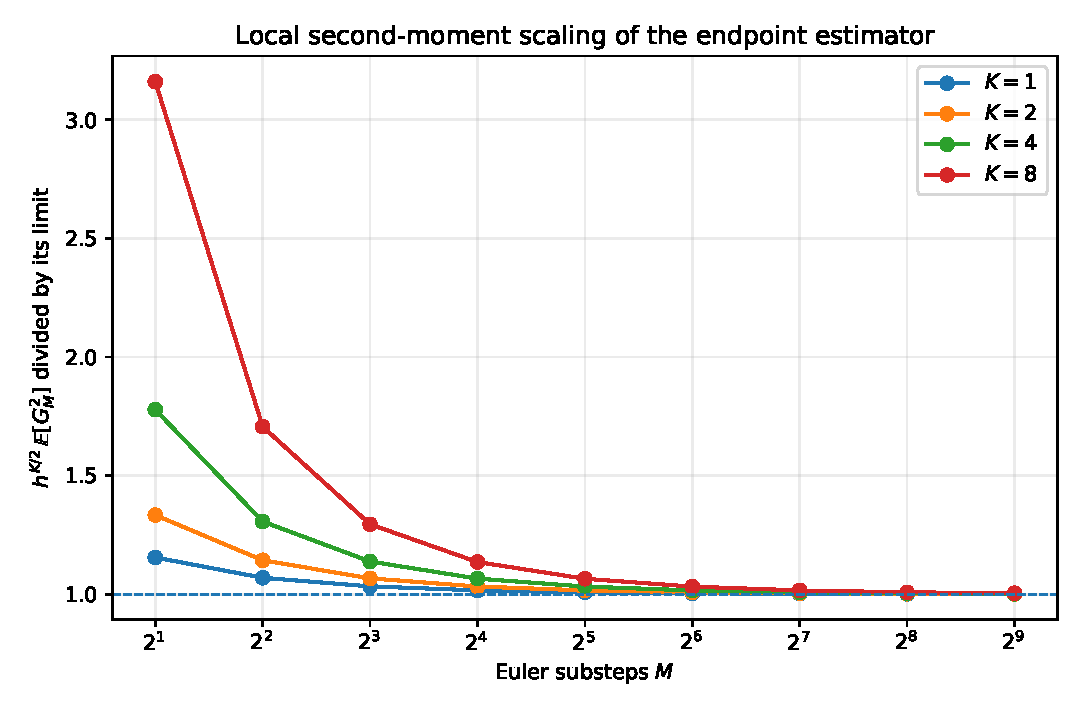
\includegraphics[width=0.86\textwidth]{figures/brownian_second_moment_scaling.pdf}
\caption{Exact local second-moment scaling for standard Brownian motion. The plotted quantity converges to one after division by its theoretical limit.}
\label{fig:brownian_scaling}
\end{figure}

\subsection{Three joint asymptotic paths}

For $K=4$, \Cref{fig:path_rmse} compares the exact relative root mean squared error under $S=M$, $S=M^2$, and $S=M^3$. The first path satisfies the published condition but has increasing RMSE. The second keeps the effective endpoint size constant and does not become consistent. The third satisfies $S/M^2\to\infty$ and has decreasing RMSE.

\begin{figure}[t]
\centering
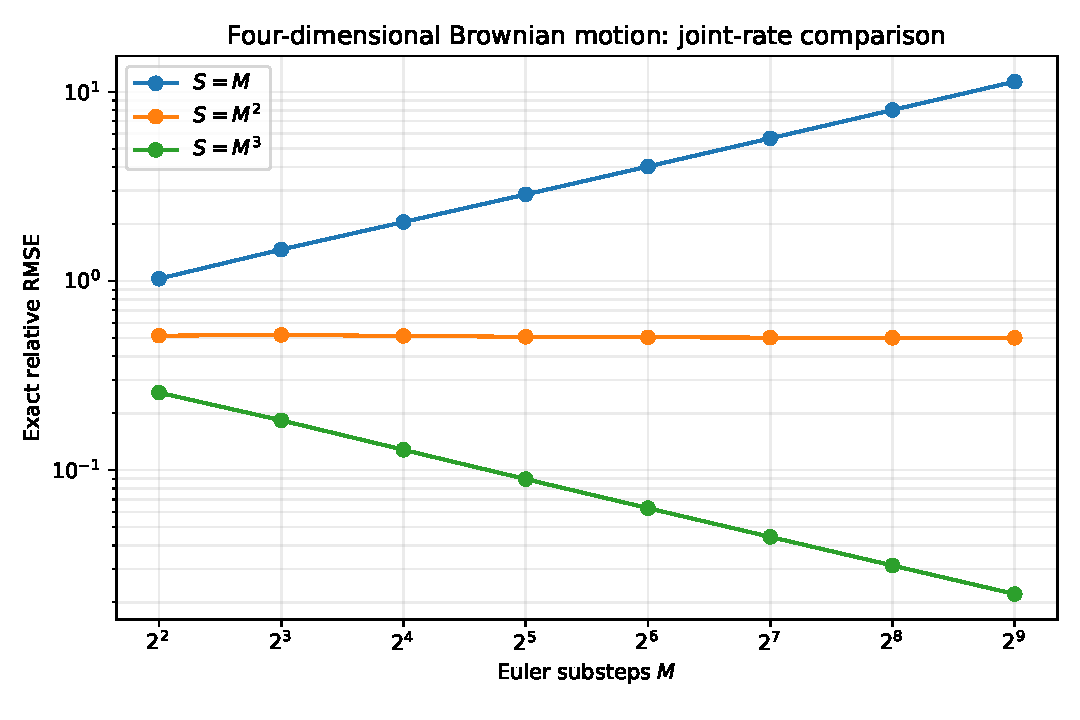
\includegraphics[width=0.86\textwidth]{figures/brownian_joint_path_rmse.pdf}
\caption{Exact relative RMSE at the origin for four-dimensional Brownian motion.}
\label{fig:path_rmse}
\end{figure}

\subsection{Typical estimates collapse while the mean remains correct}

\Cref{fig:collapse_simulation} simulates the counterexample path $M=S$. The sample median falls rapidly towards zero, and by $M=512$ more than $95\%$ of estimates are below half the true density. The sample mean remains near one after normalisation because a small number of very large realisations carry the expectation.

\begin{figure}[t]
\centering
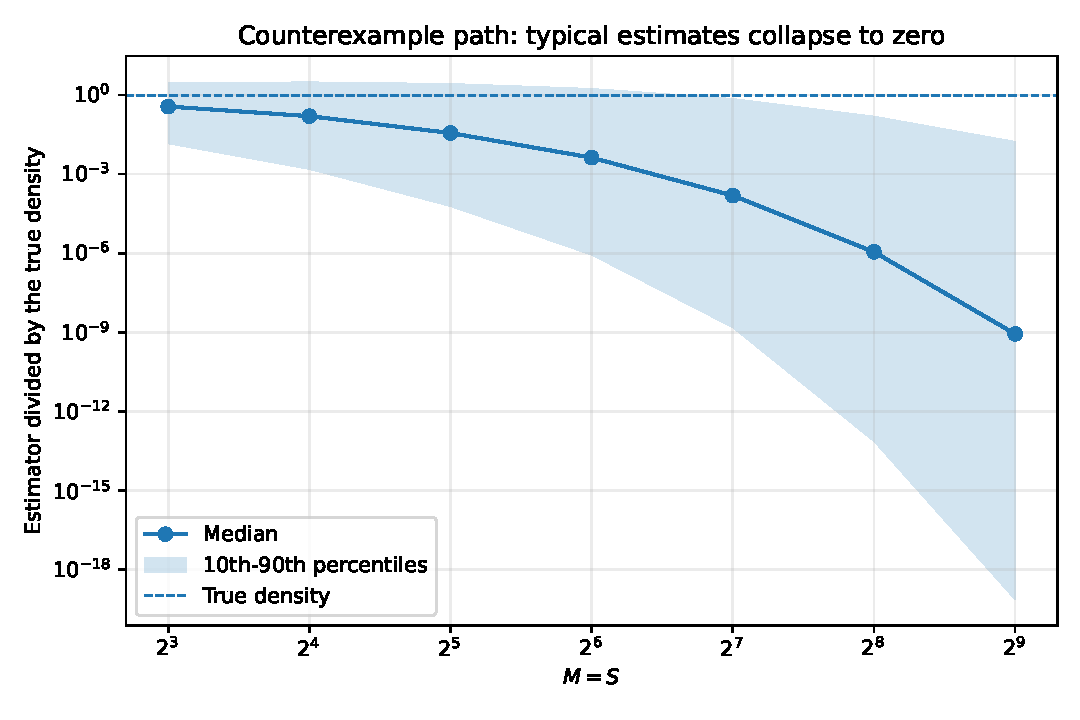
\includegraphics[width=0.86\textwidth]{figures/brownian_subcritical_distribution.pdf}
\caption{Monte Carlo distribution along $M=S$ for four-dimensional Brownian motion. Values are divided by the true density. The dashed line is one.}
\label{fig:collapse_simulation}
\end{figure}

\begin{table}[t]
\centering
\caption{Simulation of the four-dimensional Brownian counterexample path $M=S$. The estimator is divided by the true density.}
\label{tab:collapse_stats}
\small
\begin{tabular}{rrrrrrr}
\toprule
$M$ & Replications & Mean & Median & 10th pct. & 90th pct. & $\Pp(\widehat q<0.5p)$ \\
\midrule
8   & 20000 & 1.001 & 0.3674 & $1.427\times10^{-2}$ & 2.940 & 0.560 \\
16  & 20000 & 1.009 & 0.1582 & $1.520\times10^{-3}$ & 3.161 & 0.665 \\
32  & 20000 & 1.027 & 0.03628 & $5.925\times10^{-5}$ & 2.746 & 0.754 \\
64  & 20000 & 1.002 & 0.004223 & $8.507\times10^{-7}$ & 1.777 & 0.827 \\
128 & 20000 & 1.042 & $1.537\times10^{-4}$ & $1.487\times10^{-9}$ & 0.7409 & 0.886 \\
256 & 19531 & 0.941 & $1.118\times10^{-6}$ & $7.168\times10^{-14}$ & 0.1579 & 0.929 \\
512 & 9765  & 0.998 & $8.604\times10^{-10}$ & $7.076\times10^{-20}$ & 0.01738 & 0.955 \\
\bottomrule
\end{tabular}
\end{table}

\subsection{A nonzero drift does not remove the dimensional law}

Consider the diagonal Ornstein--Uhlenbeck process
\[
dY_t=-Y_tdt+dW_t
\]
in four dimensions. Its exact transition density is known, and the preterminal Euler state is Gaussian, so the second moment of the endpoint estimator can again be computed exactly. \Cref{fig:ou_scaling} shows convergence to the same local constant in \Cref{thm:local_moments}. The phenomenon is therefore not specific to driftless Brownian motion.

\begin{figure}[t]
\centering
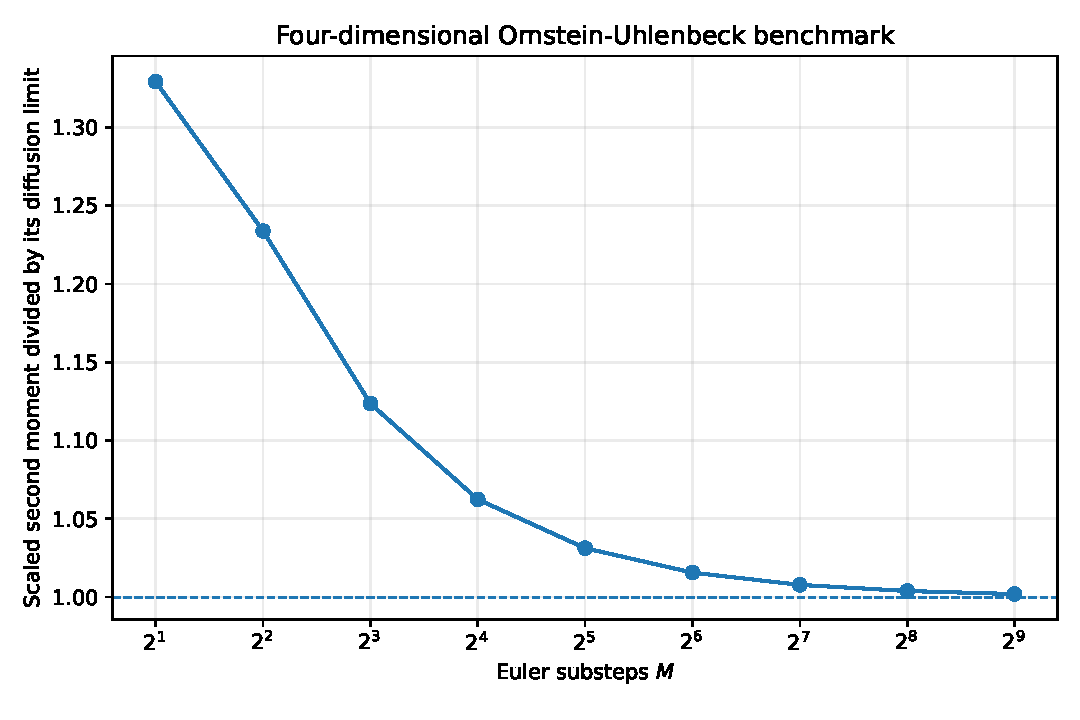
\includegraphics[width=0.86\textwidth]{figures/ou_second_moment_scaling.pdf}
\caption{Scaled second moment for a four-dimensional Ornstein--Uhlenbeck diffusion.}
\label{fig:ou_scaling}
\end{figure}

\subsection{Euler boundary violations in the incompleteness process}

\Cref{fig:negative_euler} evaluates \eqref{eq:negative_prob} using the reported estimates $(\alpha,\beta)=(0.320,0.088)$ and $(0.338,0.101)$. Even with relatively fine steps, an ordinary Euler chain near the attainable zero boundary can become negative with non-negligible probability. Once it does, the next square-root coefficient is not real without an additional numerical convention.

\begin{figure}[t]
\centering
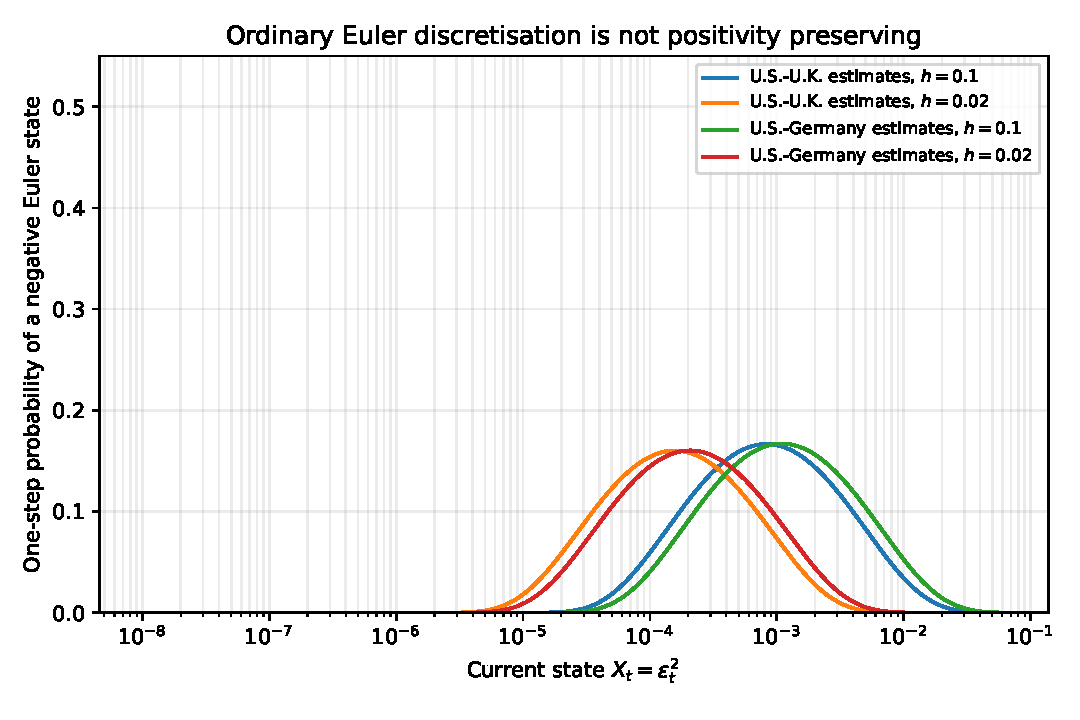
\includegraphics[width=0.86\textwidth]{figures/epsilon_squared_euler_negative_probability.pdf}
\caption{One-step probability that ordinary Euler discretisation of $X_t=\epsilon_t^2$ produces a negative state, using the estimates in Table 3 of \citet{BrandtSantaClara2002}.}
\label{fig:negative_euler}
\end{figure}

\section{Remedies and alternative constructions}\label{sec:remedies}

The endpoint variance problem is not an unavoidable property of likelihood inference for diffusions. It is a consequence of drawing preterminal states from the unconditioned forward Euler law and asking a shrinking final Gaussian kernel to connect them to a fixed observed endpoint.

\subsection{Bridge and importance proposals}

A bridge proposal guides simulated paths towards the observed endpoint. In importance-sampling language, it increases the probability of drawing paths in the region that contributes to the transition-density integral and corrects the proposal through a likelihood ratio. This is the direction taken by the acceleration methods studied by \citet{DurhamGallant2002}, conditioned-diffusion methods such as \citet{DelyonHu2006}, and later guided proposals for multidimensional bridges \citep{SchauerEtAl2017,VanDerMeulenSchauer2017}.

A useful proposal should be assessed through the moments of its importance weights. Merely changing the path simulator does not guarantee finite or dimension-stable variance, but conditioning on the endpoint directly targets the rare-event failure identified here.

\subsection{Exact or discretisation-free likelihood estimators}

For restricted classes of diffusions, exact simulation and unbiased transition-density estimators remove Euler bias entirely. \citet{BeskosEtAl2006,BeskosEtAl2009} develop likelihood-based methods of this kind. Their applicability is model dependent, but they illustrate the correct theoretical structure: unbiasedness, continuity in parameters, finite-moment conditions, and joint control of data and Monte Carlo sample sizes are stated explicitly.

\subsection{Analytical density expansions}

Closed-form expansions, such as those of \citet{AitSahalia2002}, avoid endpoint Monte Carlo variance but introduce an approximation-order problem of their own. They can be attractive for models that can be transformed to satisfy the required regularity conditions.

\subsection{Positivity-preserving discretisation}

For square-root components, ordinary Euler should be replaced by an exact transition where available or by a specified positivity-preserving approximation. The choice is part of the estimator, not an implementation detail, because different truncation and reflection rules define different transition densities.

\subsection{Practical design rule}

If the unconditioned endpoint estimator is nevertheless used, $M$ and $S$ should be calibrated jointly. A minimum diagnostic is the effective endpoint size
\[
R_{M,S}=S/M^{K/2}.
\]
Increasing $M$ without increasing $R_{M,S}$ is not an accuracy improvement. For density-level asymptotics, $R_{M,S}$ must diverge. For likelihood-level work, one should also monitor the variance and lower tail of every estimated transition density, use log-sum-exp evaluation, and verify stability after increasing both $M$ and $S$ along a theoretically admissible path.

\section{Conclusion}

The endpoint simulated-likelihood estimator has a simple but consequential dimensional structure. Its final Gaussian transition is a shrinking kernel. In $K$ dimensions, the second moment of one simulated contribution grows as $M^{K/2}$, so the Monte Carlo variance is of order $M^{K/2}/S$. The relevant simulation size is $S/M^{K/2}$.

This leads to three definite conclusions about \citet{BrandtSantaClara2002}. First, the proof of transition-density convergence combines two sequential limits without controlling their joint path. Second, the rate condition used in the asymptotic theorems is incompatible with mean-square density consistency in the four-dimensional application. Third, an exact Brownian sequence satisfying the stated condition makes the simulated density converge in probability to zero rather than to the positive true density. The issue is therefore not only a missing technical lemma; the stated joint theorem is false.

The corrected analysis also supplies constructive results. The density estimator has a triangular-array CLT under $S/M^{K/2}\to\infty$. If the Euler density bias is first order, the MSE-optimal discretisation is $M\asymp S^{2/(K+4)}$. The nonlinear log-likelihood scale is $M^{K/2}/S$, subject to the usual lower-tail conditions required for expectations of logarithms. These results explain why bridge proposals and other importance-sampling methods are not merely computational refinements: they address the rare-event geometry of the estimator.

The exchange-rate application raises separate questions. Its square-root states fall outside the smooth uniformly elliptic theory. The incompleteness state reaches a degenerate boundary and ordinary Euler is not positivity preserving. The volatility equation is implicit when risk prices depend on volatility, with the reported U.S.--U.K. estimates violating a natural sufficient condition for a unique positive branch. The Brownian correlation matrix requires a joint positive-semidefinite restriction. The final empirical estimator also contains minimum-incompleteness selection and binding constraints that are not covered by ordinary interior SML asymptotics.

None of these points, individually or collectively, proves that the finite-sample economic conclusions are false. They show that those conclusions cannot inherit the claimed maximum-likelihood asymptotics from the mathematical argument given. The appropriate post-publication response is a corrected theorem, a clear statement of the estimator actually implemented, and a re-examination of numerical stability under dimensionally valid simulation rates or bridge-based alternatives.

\appendix

\section{Additional proof details}\label{app:proofs}

\subsection{Tail control in the local moment theorem}

For completeness, suppose that $V(z)$ is globally uniformly elliptic and bounded, $\mu$ is bounded, and $r_h(z\mid x)\le C$ uniformly. Let $U$ be a neighbourhood of $y$ and let $\delta=\inf_{z\notin U}\|z-y\|>0$. For sufficiently small $h$, bounded drift gives
\[
\|y-z-h\mu(z)\|\ge\delta/2
\qquad(z\notin U).
\]
Uniform ellipticity then implies
\[
g_h(y\mid z)^r
\le C_r h^{-rK/2}\exp(-c_r/h)
\qquad(z\notin U).
\]
Multiplying by $h^{(r-1)K/2}$ and integrating against the probability density $r_h$ gives a tail bound of order $h^{-K/2}e^{-c_r/h}\to0$. This verifies the tail condition in \Cref{ass:local} under one convenient global set of assumptions.

\subsection{The Brownian collapse for more general subcritical paths}

The proof of \Cref{thm:collapse} extends beyond $M=S$. Let $h_n\downarrow0$ and choose a radius
\[
r_n=\sqrt{c h_n\log(1/h_n)}.
\]
If
\[
S_n h_n^{K/2}\{\log(1/h_n)\}^{K/2}\to0
\]
and $S_n$ grows at most polynomially in $1/h_n$, then with high probability no preterminal draw lies within $r_n$ of the endpoint, while the maximum kernel outside that ball tends to zero for sufficiently large $c$. Thus the estimator again collapses to zero. The theorem uses $M=S$ because it is transparent and directly satisfies the published rate in four dimensions.

\section{Reproducibility}\label{app:repro}

The accompanying directory contains:
\begin{itemize}
\item \texttt{main.tex}, the manuscript source;
\item \texttt{references.bib}, the bibliography;
\item \texttt{code/generate\_results.py}, the fully reproducible simulation and figure code;
\item vector PDF and PNG versions of all figures;
\item CSV and LaTeX versions of generated numerical tables.
\end{itemize}
The code uses a fixed seed, vectorised Gaussian simulation, and log-sum-exp evaluation of the endpoint estimator. No proprietary data are used.

\printbibliography

\end{document}
